%----------------------------------------------------------------------------------------
%    PACKAGES AND THEMES
%----------------------------------------------------------------------------------------
\documentclass[aspectratio=169,xcolor=dvipsnames]{beamer}
\makeatletter
\def\input@path{{../BeamerTemplate/theme/}}
\makeatother
\usetheme{CleanEasy}
\usepackage[utf8]{inputenc}
\usepackage{lmodern}
\usepackage[T1]{fontenc}
\usepackage{fix-cm}
\usepackage{amsmath}
\usepackage{mathtools}
\usepackage{listings}
\usepackage{xcolor}
\usepackage{hyperref}
\usepackage{graphicx}
\usepackage{booktabs}
\usepackage{tikz}
\usetikzlibrary{positioning, shapes, arrows, calc, decorations.pathreplacing, arrows.meta, backgrounds, patterns, overlay-beamer-styles}
\usepackage{etoolbox}

%----------------------------------------------------------------------------------------
%    LAYOUT CONFIGURATION
%----------------------------------------------------------------------------------------
\input{../BeamerTemplate/configs/configs}

%----------------------------------------------------------------------------------------
%    TITLE PAGE CONFIGURATION
%----------------------------------------------------------------------------------------
\title{Next Steps}
\subtitle{Explore Advanced and Specialized Topics to Continue Growing}
\author{Minseok Jeon}
\institute{DGIST}
\date{\today}

\begin{document}

\begin{frame}
  \titlepage
\end{frame}

\begin{frame}{Outline}
  \tableofcontents
\end{frame}

% Introduction
\section{Introduction}

\begin{frame}{Course Journey Recap}
  \textbf{What You've Learned:}
  \begin{itemize}
    \item \textbf{Foundations}: Arrays, linked lists, stacks, queues, hash tables
    \item \textbf{Trees \& Graphs}: Binary trees, BSTs, heaps, graph algorithms
    \item \textbf{Advanced Structures}: Tries, B-trees, union-find, segment trees
    \item \textbf{Algorithms}: Sorting, searching, graph traversal, dynamic programming
    \item \textbf{Applications}: Real-world projects and interview preparation
  \end{itemize}

  \vspace{0.3cm}
  \begin{block}{You're Ready!}
    You now have a solid foundation in data structures and algorithms. This lecture explores where to go next.
  \end{block}
\end{frame}

\begin{frame}{What's Next?}
  \textbf{Five Advanced Directions:}
  \begin{enumerate}
    \item \textbf{Parallel \& Distributed Data Structures}
    \begin{itemize}
      \item Multi-threaded and distributed computing
      \item Concurrent data structures, consistent hashing, CRDTs
    \end{itemize}

    \vspace{0.2cm}
    \item \textbf{Data Structures in Machine Learning}
    \begin{itemize}
      \item Tensors, graph neural networks, embeddings
      \item Specialized structures for ML workflows
    \end{itemize}

    \vspace{0.2cm}
    \item \textbf{Persistent \& Functional Data Structures}
    \begin{itemize}
      \item Immutable structures, version control
      \item Used in functional programming languages
    \end{itemize}

    \vspace{0.2cm}
    \item \textbf{External Memory \& Cache-Oblivious Structures}
    \begin{itemize}
      \item Optimizing for disk I/O and memory hierarchy
      \item B-trees, LSM trees, cache-aware algorithms
    \end{itemize}

    \vspace{0.2cm}
    \item \textbf{Reading Research Papers \& Implementations}
    \begin{itemize}
      \item Learning cutting-edge techniques
      \item Implementing from academic papers
    \end{itemize}
  \end{enumerate}
\end{frame}

% Parallel and Distributed Data Structures
\section{Parallel \& Distributed Data Structures}

\begin{frame}{Why Parallel \& Distributed?}
  \begin{columns}
    \begin{column}{0.5\textwidth}
      \textbf{Motivation:}
      \begin{itemize}
        \item Modern CPUs have multiple cores
        \item Big data requires distributed systems
        \item Single-threaded = leaving performance on table
        \item Cloud computing is inherently distributed
      \end{itemize}

      \vspace{0.3cm}
      \textbf{Challenges:}
      \begin{itemize}
        \item Race conditions
        \item Deadlocks
        \item Data consistency
        \item Network failures
      \end{itemize}
    \end{column}

    \begin{column}{0.5\textwidth}
      \textbf{Examples:}
      \begin{itemize}
        \item Multi-threaded web servers
        \item Distributed databases (Cassandra, MongoDB)
        \item MapReduce frameworks (Hadoop, Spark)
        \item P2P networks (BitTorrent, blockchain)
      \end{itemize}

      \vspace{0.3cm}
      \textbf{Goal:}
      \begin{itemize}
        \item Safe concurrency
        \item Scalability across machines
        \item Fault tolerance
      \end{itemize}
    \end{column}
  \end{columns}
\end{frame}

\subsection{Concurrent Data Structures}

\begin{frame}{Concurrent Data Structures}
  \textbf{Thread-Safe Implementations:}

  \vspace{0.3cm}
  \begin{itemize}
    \item \textbf{Lock-Free Structures}
    \begin{itemize}
      \item Use atomic operations (CAS - Compare-And-Swap)
      \item No threads block waiting for locks
      \item Example: Lock-free queue, lock-free stack
      \item Complexity: Higher implementation complexity, better throughput
    \end{itemize}

    \vspace{0.2cm}
    \item \textbf{Concurrent Hash Maps}
    \begin{itemize}
      \item Java's \texttt{ConcurrentHashMap}: Lock striping (segment-level locks)
      \item C++ concurrent containers: \texttt{std::concurrent\_*}
      \item Fine-grained locking for better concurrency
    \end{itemize}

    \vspace{0.2cm}
    \item \textbf{Read-Write Locks}
    \begin{itemize}
      \item Multiple readers, single writer
      \item Reader-writer problem solution
      \item Use case: Read-heavy workloads (caches, databases)
    \end{itemize}

    \vspace{0.2cm}
    \item \textbf{Producer-Consumer Queues}
    \begin{itemize}
      \item Bounded/unbounded blocking queues
      \item Multiple producers, multiple consumers
      \item Use case: Task scheduling, work distribution
    \end{itemize}
  \end{itemize}
\end{frame}

\begin{frame}{Lock-Free Queue Example}
  \begin{center}
    \textbf{Lock-Free Queue using CAS:}

    \vspace{0.3cm}
    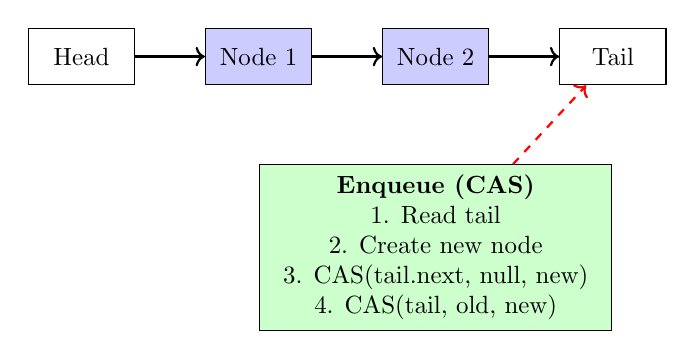
\begin{tikzpicture}[scale=0.9, every node/.style={scale=0.9}]
      % Queue nodes
      \node[draw, rectangle, minimum width=1.5cm, minimum height=0.8cm] (head) at (0, 0) {Head};
      \node[draw, rectangle, minimum width=1.5cm, minimum height=0.8cm, fill=blue!20] (n1) at (2.5, 0) {Node 1};
      \node[draw, rectangle, minimum width=1.5cm, minimum height=0.8cm, fill=blue!20] (n2) at (5, 0) {Node 2};
      \node[draw, rectangle, minimum width=1.5cm, minimum height=0.8cm] (tail) at (7.5, 0) {Tail};

      % Arrows
      \draw[->, thick] (head) -- (n1);
      \draw[->, thick] (n1) -- (n2);
      \draw[->, thick] (n2) -- (tail);

      % CAS operation
      \node[below=1cm of n2, draw, rectangle, fill=green!20, minimum width=3cm] (cas) {
        \begin{tabular}{c}
          \textbf{Enqueue (CAS)} \\
          1. Read tail \\
          2. Create new node \\
          3. CAS(tail.next, null, new) \\
          4. CAS(tail, old, new)
        \end{tabular}
      };

      \draw[->, dashed, thick, red] (cas) -- (tail);
    \end{tikzpicture}
  \end{center}

  \vspace{0.3cm}
  \textbf{Key Idea:}
  \begin{itemize}
    \item Atomic CAS ensures no two threads modify same location simultaneously
    \item Retry on CAS failure (optimistic concurrency)
    \item No locks $\to$ no deadlocks, better scalability
  \end{itemize}
\end{frame}

\subsection{Distributed Data Structures}

\begin{frame}{Distributed Hash Tables (DHT)}
  \begin{columns}
    \begin{column}{0.5\textwidth}
      \textbf{Concept:}
      \begin{itemize}
        \item Hash table across multiple machines
        \item Decentralized, no single point of failure
        \item Each node responsible for key range
      \end{itemize}

      \vspace{0.3cm}
      \textbf{Algorithms:}
      \begin{itemize}
        \item \textbf{Chord}: Ring topology, $O(\log n)$ lookup
        \item \textbf{Kademlia}: XOR metric, used in BitTorrent
        \item \textbf{Consistent Hashing}: Load balancing
      \end{itemize}
    \end{column}

    \begin{column}{0.5\textwidth}
      \textbf{Consistent Hashing:}
      \begin{itemize}
        \item Map keys and nodes to ring
        \item Key stored on next node clockwise
        \item Adding/removing nodes affects only neighbors
        \item Used in: Memcached, Redis Cluster, Cassandra
      \end{itemize}

      \vspace{0.3cm}
      \textbf{Benefits:}
      \begin{itemize}
        \item Minimal key redistribution on node changes
        \item Fault tolerance
        \item Horizontal scalability
      \end{itemize}
    \end{column}
  \end{columns}
\end{frame}

\begin{frame}{Consistent Hashing Visualization}
  \begin{center}
    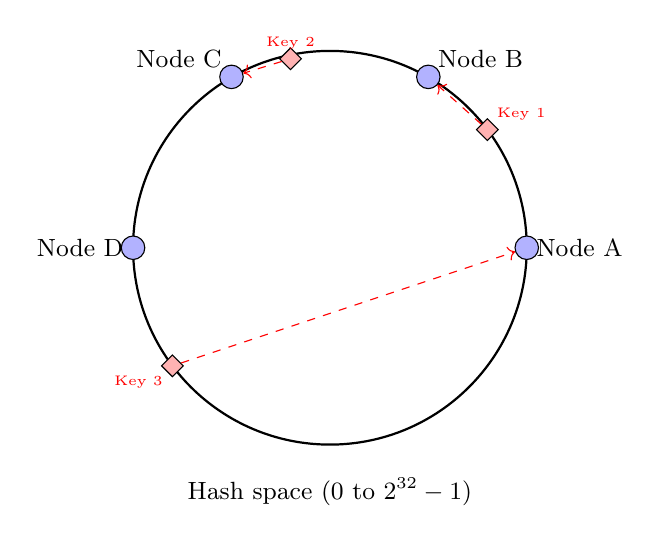
\begin{tikzpicture}[scale=1.0]
      % Circle
      \draw[thick] (0, 0) circle (2.5cm);

      % Nodes
      \node[draw, circle, fill=blue!30, inner sep=3pt] (n1) at (2.5, 0) {};
      \node[right] at (n1) {\small Node A};

      \node[draw, circle, fill=blue!30, inner sep=3pt] (n2) at (1.25, 2.17) {};
      \node[above right] at (n2) {\small Node B};

      \node[draw, circle, fill=blue!30, inner sep=3pt] (n3) at (-1.25, 2.17) {};
      \node[above left] at (n3) {\small Node C};

      \node[draw, circle, fill=blue!30, inner sep=3pt] (n4) at (-2.5, 0) {};
      \node[left] at (n4) {\small Node D};

      % Keys
      \node[draw, diamond, fill=red!30, inner sep=2pt] (k1) at (2, 1.5) {};
      \node[above right, red] at (k1) {\tiny Key 1};

      \node[draw, diamond, fill=red!30, inner sep=2pt] (k2) at (-0.5, 2.4) {};
      \node[above, red] at (k2) {\tiny Key 2};

      \node[draw, diamond, fill=red!30, inner sep=2pt] (k3) at (-2, -1.5) {};
      \node[below left, red] at (k3) {\tiny Key 3};

      % Arrows showing key assignment
      \draw[->, dashed, red] (k1) -- (n2);
      \draw[->, dashed, red] (k2) -- (n3);
      \draw[->, dashed, red] (k3) -- (n1);

      % Ring label
      \node[below=2.8cm of {(0,0)}] {\small Hash space (0 to $2^{32}-1$)};
    \end{tikzpicture}
  \end{center}

  \textbf{Key Assignment:} Each key assigned to first node clockwise on ring
\end{frame}

\begin{frame}{CRDTs: Conflict-Free Replicated Data Types}
  \begin{columns}
    \begin{column}{0.5\textwidth}
      \textbf{Concept:}
      \begin{itemize}
        \item Designed for eventual consistency
        \item No coordination needed
        \item Merging replicas is commutative \& associative
        \item Guaranteed convergence
      \end{itemize}

      \vspace{0.3cm}
      \textbf{Types:}
      \begin{itemize}
        \item \textbf{G-Counter}: Grow-only counter
        \item \textbf{PN-Counter}: Increment/decrement counter
        \item \textbf{G-Set}: Grow-only set
        \item \textbf{OR-Set}: Observed-Remove set
        \item \textbf{LWW-Register}: Last-Write-Wins register
      \end{itemize}
    \end{column}

    \begin{column}{0.5\textwidth}
      \textbf{Example: G-Counter}
      \begin{itemize}
        \item Each replica has array of counts (one per node)
        \item Increment updates local count
        \item Merge takes element-wise max
        \item Value = sum of all counts
      \end{itemize}

      \vspace{0.3cm}
      \textbf{Applications:}
      \begin{itemize}
        \item Collaborative editing (Google Docs)
        \item Distributed databases (Riak, Redis)
        \item Real-time synchronization
        \item Mobile apps with offline support
      \end{itemize}
    \end{column}
  \end{columns}

  \vspace{0.3cm}
  \begin{block}{Key Property}
    CRDTs achieve strong eventual consistency without consensus protocols
  \end{block}
\end{frame}

\subsection{Parallel Algorithms}

\begin{frame}{Parallel Algorithms Overview}
  \begin{columns}
    \begin{column}{0.5\textwidth}
      \textbf{Parallel Sorting:}
      \begin{itemize}
        \item \textbf{Parallel Merge Sort}: Divide array, sort in parallel, merge
        \item \textbf{Parallel Quick Sort}: Partition in parallel, recurse
        \item Fork-Join framework (Java, C++)
        \item Speedup: Near-linear with number of cores
      \end{itemize}

      \vspace{0.3cm}
      \textbf{Parallel Prefix Sum:}
      \begin{itemize}
        \item Tree-based reduction
        \item Applications: Stream compaction, radix sort
        \item GPU-friendly (CUDA, OpenCL)
      \end{itemize}
    \end{column}

    \begin{column}{0.5\textwidth}
      \textbf{MapReduce Paradigm:}
      \begin{itemize}
        \item \textbf{Map}: Process data in parallel
        \item \textbf{Reduce}: Aggregate results
        \item Frameworks: Hadoop, Spark
      \end{itemize}

      \vspace{0.3cm}
      \textbf{Example: Word Count}
      \begin{enumerate}
        \item Map: (doc $\to$ (word, 1) pairs)
        \item Shuffle: Group by word
        \item Reduce: Sum counts per word
      \end{enumerate}

      \vspace{0.3cm}
      \textbf{Synchronization:}
      \begin{itemize}
        \item Barriers for phase sync
        \item Atomic operations
        \item Memory fences
      \end{itemize}
    \end{column}
  \end{columns}
\end{frame}

% Data Structures in ML
\section{Data Structures in Machine Learning}

\begin{frame}{ML Data Structures Landscape}
  \textbf{Why Specialized Structures?}
  \begin{itemize}
    \item Machine learning operates on high-dimensional data
    \item Computational efficiency is critical (training time, inference latency)
    \item Memory optimization for large models and datasets
    \item Specialized hardware (GPUs, TPUs) requires specific layouts
  \end{itemize}

  \vspace{0.3cm}
  \textbf{Key Structures:}
  \begin{enumerate}
    \item \textbf{Tensors}: Multi-dimensional arrays for neural networks
    \item \textbf{Graph Structures}: For graph neural networks
    \item \textbf{Embeddings}: Nearest neighbor search in high dimensions
    \item \textbf{Batch Processing}: Efficient data loading and preprocessing
  \end{enumerate}
\end{frame}

\subsection{Tensors}

\begin{frame}{Tensors: Multi-Dimensional Arrays}
  \begin{columns}
    \begin{column}{0.5\textwidth}
      \textbf{Definition:}
      \begin{itemize}
        \item Generalization of vectors and matrices
        \item 0D: Scalar
        \item 1D: Vector
        \item 2D: Matrix
        \item 3D+: Tensor
      \end{itemize}

      \vspace{0.3cm}
      \textbf{Example: Image Tensor}
      \begin{itemize}
        \item Shape: (batch, channels, height, width)
        \item (32, 3, 224, 224) = 32 RGB images of 224x224
        \item Memory: 32 $\times$ 3 $\times$ 224 $\times$ 224 $\times$ 4 bytes $\approx$ 19 MB
      \end{itemize}
    \end{column}

    \begin{column}{0.5\textwidth}
      \textbf{Storage Formats:}
      \begin{itemize}
        \item \textbf{Row-major (C-style)}: Last index varies fastest
        \item \textbf{Column-major (Fortran)}: First index varies fastest
        \item Affects cache performance
      \end{itemize}

      \vspace{0.3cm}
      \textbf{Operations:}
      \begin{itemize}
        \item Broadcasting: Automatic dimension matching
        \item Reshaping: Change dimensions without copying
        \item Slicing: Extract subtensors
        \item Element-wise ops: Add, multiply, etc.
      \end{itemize}

      \vspace{0.3cm}
      \textbf{Frameworks:}
      \begin{itemize}
        \item NumPy, PyTorch, TensorFlow, JAX
      \end{itemize}
    \end{column}
  \end{columns}
\end{frame}

\begin{frame}{Sparse Tensors}
  \begin{columns}
    \begin{column}{0.5\textwidth}
      \textbf{Motivation:}
      \begin{itemize}
        \item Many tensors are sparse (mostly zeros)
        \item Example: Embeddings, text data, graphs
        \item Dense storage wasteful
      \end{itemize}

      \vspace{0.3cm}
      \textbf{COO Format (Coordinate):}
      \begin{itemize}
        \item Store: (indices, values)
        \item Example: (0,2): 5, (1,1): 3, (2,0): 7
        \item Good for: Construction, random access
      \end{itemize}
    \end{column}

    \begin{column}{0.5\textwidth}
      \textbf{CSR Format (Compressed Sparse Row):}
      \begin{itemize}
        \item Store: row\_ptr, col\_indices, values
        \item More memory efficient than COO
        \item Fast row access
        \item Used in: Matrix multiplication, graph algorithms
      \end{itemize}

      \vspace{0.3cm}
      \textbf{Example: 3x3 Sparse Matrix}
      \[
      \begin{bmatrix}
      0 & 0 & 5 \\
      0 & 3 & 0 \\
      7 & 0 & 0
      \end{bmatrix}
      \]

      CSR: \\
      row\_ptr = [0, 1, 2, 3] \\
      col\_indices = [2, 1, 0] \\
      values = [5, 3, 7]
    \end{column}
  \end{columns}
\end{frame}

\subsection{Graph Neural Networks}

\begin{frame}{GNN Graph Representations}
  \begin{columns}
    \begin{column}{0.5\textwidth}
      \textbf{Adjacency Matrix:}
      \begin{itemize}
        \item Dense $O(V^2)$ representation
        \item Fast edge queries: $O(1)$
        \item Good for: Dense graphs, small graphs
        \item Matrix multiplication for message passing
      \end{itemize}

      \vspace{0.3cm}
      \textbf{Adjacency List:}
      \begin{itemize}
        \item Sparse representation
        \item Space: $O(V + E)$
        \item Good for: Sparse graphs (most real-world)
        \item Iteration over neighbors: $O(\text{degree})$
      \end{itemize}
    \end{column}

    \begin{column}{0.5\textwidth}
      \textbf{Edge List:}
      \begin{itemize}
        \item Simple (source, target, weight) tuples
        \item Easy to store and load
        \item Requires sorting for efficient queries
      \end{itemize}

      \vspace{0.3cm}
      \textbf{Libraries:}
      \begin{itemize}
        \item \textbf{NetworkX}: Python graph library
        \item \textbf{PyTorch Geometric}: GNN framework
        \item \textbf{DGL}: Deep Graph Library
        \item \textbf{GraphSAGE, GCN}: Message passing
      \end{itemize}

      \vspace{0.3cm}
      \textbf{Applications:}
      \begin{itemize}
        \item Social networks
        \item Molecular structures
        \item Recommendation systems
      \end{itemize}
    \end{column}
  \end{columns}
\end{frame}

\subsection{Embeddings and Search}

\begin{frame}{Embedding Structures}
  \begin{columns}
    \begin{column}{0.5\textwidth}
      \textbf{Embedding Tables:}
      \begin{itemize}
        \item Lookup table for categorical features
        \item Maps discrete IDs to dense vectors
        \item Example: Word embeddings (word $\to$ 300D vector)
        \item Learned during training
      \end{itemize}

      \vspace{0.3cm}
      \textbf{Nearest Neighbor Search:}
      \begin{itemize}
        \item Find similar embeddings
        \item Exact: Brute force $O(n)$
        \item Approximate: Much faster, slight accuracy loss
      \end{itemize}
    \end{column}

    \begin{column}{0.5\textwidth}
      \textbf{Search Structures:}
      \begin{itemize}
        \item \textbf{KD-Trees}: $O(\log n)$ for low dimensions ($d < 20$)
        \item \textbf{Ball Trees}: Better for higher dimensions
        \item \textbf{HNSW}: Hierarchical Navigable Small World
        \begin{itemize}
          \item Graph-based approximate search
          \item Very fast: $O(\log n)$ queries
        \end{itemize}
        \item \textbf{FAISS}: Facebook's similarity search library
        \begin{itemize}
          \item GPU acceleration
          \item Billions of vectors
        \end{itemize}
      \end{itemize}

      \vspace{0.3cm}
      \textbf{Use Cases:}
      \begin{itemize}
        \item Recommendation engines
        \item Image search
        \item Semantic search
      \end{itemize}
    \end{column}
  \end{columns}
\end{frame}

% Persistent and Functional Data Structures
\section{Persistent \& Functional Data Structures}

\begin{frame}{Persistence: Preserving History}
  \begin{block}{Definition}
    Persistent data structures preserve previous versions after modifications
  \end{block}

  \vspace{0.3cm}
  \textbf{Types of Persistence:}
  \begin{itemize}
    \item \textbf{Ephemeral}: Standard mutable structures (old version destroyed)
    \item \textbf{Partially Persistent}: Access all versions, modify only latest
    \item \textbf{Fully Persistent}: Access and modify any version
    \item \textbf{Confluently Persistent}: Merge different versions
  \end{itemize}

  \vspace{0.3cm}
  \textbf{Benefits:}
  \begin{itemize}
    \item Undo/redo functionality
    \item Version control systems
    \item Concurrent programming without locks
    \item Functional programming paradigm
  \end{itemize}
\end{frame}

\begin{frame}{Persistent Lists: Structural Sharing}
  \begin{center}
    \textbf{Linked List with Sharing:}

    \vspace{0.3cm}
    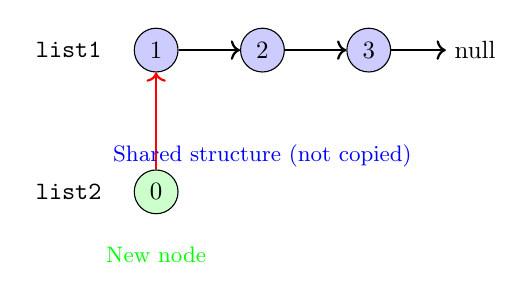
\begin{tikzpicture}[scale=0.9, every node/.style={scale=0.9}]
      % Original list
      \node[draw, circle, fill=blue!20] (a1) at (0, 2) {1};
      \node[draw, circle, fill=blue!20] (a2) at (1.5, 2) {2};
      \node[draw, circle, fill=blue!20] (a3) at (3, 2) {3};
      \node (anull) at (4.5, 2) {null};

      \draw[->, thick] (a1) -- (a2);
      \draw[->, thick] (a2) -- (a3);
      \draw[->, thick] (a3) -- (anull);

      \node[left=0.3cm of a1] {\texttt{list1}};

      % New list sharing structure
      \node[draw, circle, fill=green!20] (b0) at (0, 0) {0};
      \draw[->, thick, red] (b0) -- (a1);

      \node[left=0.3cm of b0] {\texttt{list2}};

      % Annotations
      \node[below=0.8cm of a2, font=\small, blue] {Shared structure (not copied)};
      \node[below=0.3cm of b0, font=\small, green] {New node};
    \end{tikzpicture}
  \end{center}

  \vspace{0.3cm}
  \textbf{Key Idea:}
  \begin{itemize}
    \item \texttt{list1 = [1, 2, 3]}
    \item \texttt{list2 = cons(0, list1) = [0, 1, 2, 3]}
    \item Both lists coexist, sharing nodes [1, 2, 3]
    \item Time: $O(1)$ for cons, Space: $O(1)$ per operation
  \end{itemize}
\end{frame}

\begin{frame}{Persistent Trees: Path Copying}
  \begin{center}
    \textbf{Updating a Red-Black Tree:}

    \vspace{0.3cm}
    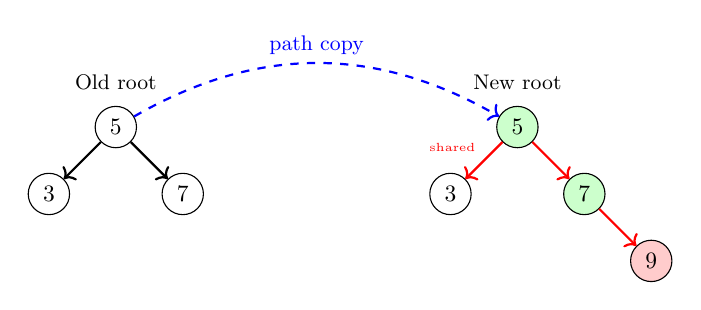
\begin{tikzpicture}[scale=0.85, every node/.style={scale=0.85}]
      % Original tree
      \node[draw, circle] (r1) at (-3, 2) {5};
      \node[draw, circle] (l1) at (-4, 1) {3};
      \node[draw, circle] (r1r) at (-2, 1) {7};

      \draw[->, thick] (r1) -- (l1);
      \draw[->, thick] (r1) -- (r1r);

      \node[above=0.1cm of r1] {\small Old root};

      % New tree (after insert)
      \node[draw, circle, fill=green!20] (r2) at (3, 2) {5};
      \node[draw, circle] (l2) at (2, 1) {3};  % Shared
      \node[draw, circle, fill=green!20] (r2r) at (4, 1) {7};
      \node[draw, circle, fill=red!20] (r2rr) at (5, 0) {9};  % New

      \draw[->, thick, red] (r2) -- (l2) node[midway, above left, font=\tiny] {shared};
      \draw[->, thick, red] (r2) -- (r2r);
      \draw[->, thick, red] (r2r) -- (r2rr);

      \node[above=0.1cm of r2] {\small New root};

      % Arrow showing copy
      \draw[->, dashed, thick, blue] (r1) to[bend left] node[midway, above] {\small path copy} (r2);
    \end{tikzpicture}
  \end{center}

  \vspace{0.3cm}
  \textbf{Path Copying:}
  \begin{itemize}
    \item Copy only nodes on path from root to modified node
    \item Other subtrees shared (not copied)
    \item Time: $O(\log n)$ per operation, Space: $O(\log n)$ per version
    \item Old version still accessible through old root
  \end{itemize}
\end{frame}

\begin{frame}{Persistent Hash Maps: HAMT}
  \begin{columns}
    \begin{column}{0.5\textwidth}
      \textbf{Hash Array Mapped Trie (HAMT):}
      \begin{itemize}
        \item Used in Clojure, Scala
        \item 32-way branching tree
        \item Hash bits determine path
        \item Efficient updates with sharing
      \end{itemize}

      \vspace{0.3cm}
      \textbf{Structure:}
      \begin{itemize}
        \item Root has 32 children (5 bits of hash)
        \item Each level consumes 5 bits
        \item Depth: $\lceil \log_{32} n \rceil$
      \end{itemize}
    \end{column}

    \begin{column}{0.5\textwidth}
      \textbf{Persistent Vectors:}
      \begin{itemize}
        \item Clojure's persistent vector
        \item 32-way branching tree
        \item $O(\log_{32} n) \approx O(1)$ for practical sizes
        \item Efficient append, update, lookup
      \end{itemize}

      \vspace{0.3cm}
      \textbf{Complexity:}
      \begin{itemize}
        \item Lookup: $O(\log_{32} n)$
        \item Update: $O(\log_{32} n)$
        \item Append: $O(\log_{32} n)$
        \item For $n < 32^6 \approx 10^9$: $\le 6$ operations
      \end{itemize}
    \end{column}
  \end{columns}

  \vspace{0.3cm}
  \begin{block}{Applications}
    Functional programming languages, concurrent systems, version control
  \end{block}
\end{frame}

% External Memory and Cache-Oblivious
\section{External Memory \& Cache-Oblivious Structures}

\begin{frame}{Memory Hierarchy Reality}
  \begin{columns}
    \begin{column}{0.5\textwidth}
      \textbf{Memory Hierarchy:}
      \begin{itemize}
        \item L1 Cache: 64 KB, 1 ns
        \item L2 Cache: 256 KB, 4 ns
        \item L3 Cache: 8 MB, 10 ns
        \item RAM: 16 GB, 100 ns
        \item SSD: 512 GB, 100 $\mu$s
        \item HDD: 2 TB, 10 ms
      \end{itemize}

      \vspace{0.3cm}
      \textbf{Gap:}
      \begin{itemize}
        \item RAM is 100x slower than L1
        \item Disk is 100,000x slower than RAM
        \item I/O is the bottleneck
      \end{itemize}
    \end{column}

    \begin{column}{0.5\textwidth}
      \textbf{External Memory Model:}
      \begin{itemize}
        \item Data stored on disk
        \item Limited RAM (cache)
        \item Transfer data in blocks
        \item Goal: Minimize I/O operations
      \end{itemize}

      \vspace{0.3cm}
      \textbf{Cost Model:}
      \begin{itemize}
        \item Count block reads/writes
        \item Ignore in-memory computation
        \item Block size: $B$ elements
        \item Memory size: $M$ elements
      \end{itemize}

      \vspace{0.3cm}
      \textbf{Why Care?}
      \begin{itemize}
        \item Big data doesn't fit in RAM
        \item Databases on disk
        \item Cache performance critical
      \end{itemize}
    \end{column}
  \end{columns}
\end{frame}

\subsection{B-Trees for External Memory}

\begin{frame}{B-Trees: Disk-Optimized Trees}
  \begin{columns}
    \begin{column}{0.5\textwidth}
      \textbf{Design for Disk:}
      \begin{itemize}
        \item High branching factor (100-1000)
        \item Each node = one disk block
        \item Shallow tree (minimize I/Os)
        \item All leaves at same level
      \end{itemize}

      \vspace{0.3cm}
      \textbf{Example:}
      \begin{itemize}
        \item Branching factor $B = 100$
        \item Height: $\log_{100} n$
        \item For $n = 1$ billion: height $\approx 5$
        \item 5 disk reads for any query!
      \end{itemize}
    \end{column}

    \begin{column}{0.5\textwidth}
      \textbf{Operations:}
      \begin{itemize}
        \item Search: $O(\log_B n)$ I/Os
        \item Insert: $O(\log_B n)$ I/Os
        \item Delete: $O(\log_B n)$ I/Os
        \item Range query: $O(\log_B n + k/B)$ I/Os
      \end{itemize}

      \vspace{0.3cm}
      \textbf{B+ Trees:}
      \begin{itemize}
        \item All data in leaves
        \item Internal nodes only keys
        \item Leaves linked (range queries)
        \item Used in: Databases (MySQL, PostgreSQL)
      \end{itemize}

      \vspace{0.3cm}
      \textbf{File Systems:}
      \begin{itemize}
        \item ext4, NTFS, Btrfs use B-trees
      \end{itemize}
    \end{column}
  \end{columns}
\end{frame}

\subsection{LSM Trees}

\begin{frame}{LSM Trees: Write-Optimized Structures}
  \begin{columns}
    \begin{column}{0.5\textwidth}
      \textbf{Log-Structured Merge Trees:}
      \begin{itemize}
        \item Optimized for write-heavy workloads
        \item Used in: LevelDB, RocksDB, Cassandra, HBase
        \item Trade read performance for write throughput
      \end{itemize}

      \vspace{0.3cm}
      \textbf{Structure:}
      \begin{itemize}
        \item \textbf{Memtable}: In-memory sorted map
        \item \textbf{SSTables}: Immutable sorted files on disk
        \item Levels of increasing size (10x each level)
      \end{itemize}
    \end{column}

    \begin{column}{0.5\textwidth}
      \textbf{Operations:}
      \begin{itemize}
        \item \textbf{Write}: Insert into memtable ($O(\log n)$)
        \item When full: Flush memtable to SSTable
        \item \textbf{Read}: Check memtable, then SSTables (bloom filter helps)
        \item \textbf{Compaction}: Merge SSTables periodically
      \end{itemize}

      \vspace{0.3cm}
      \textbf{Benefits:}
      \begin{itemize}
        \item Fast writes (sequential I/O)
        \item Good compression
        \item No fragmentation
      \end{itemize}

      \vspace{0.3cm}
      \textbf{Drawbacks:}
      \begin{itemize}
        \item Slower reads
        \item Write amplification (compaction)
      \end{itemize}
    \end{column}
  \end{columns}
\end{frame}

\subsection{Cache-Oblivious Algorithms}

\begin{frame}{Cache-Oblivious Algorithms}
  \begin{block}{Definition}
    Algorithms optimal for all levels of memory hierarchy without knowing cache parameters ($B$, $M$)
  \end{block}

  \vspace{0.3cm}
  \textbf{Key Idea:}
  \begin{itemize}
    \item Recursive divide-and-conquer
    \item Eventually fits in cache
    \item Automatically adapts to any cache size
  \end{itemize}

  \vspace{0.3cm}
  \textbf{Examples:}
  \begin{itemize}
    \item \textbf{Funnelsort}: Cache-oblivious sorting
    \begin{itemize}
      \item $O(N/B \log_{M/B} N/B)$ I/Os (optimal)
      \item Recursive merging with "funnels"
    \end{itemize}
    \item \textbf{Van Emde Boas Layout}: Tree layout for cache efficiency
    \begin{itemize}
      \item Recursive decomposition
      \item Better cache performance than level-order
    \end{itemize}
    \item \textbf{Matrix Multiplication}: Recursive blocking
    \begin{itemize}
      \item Divide matrices into quadrants
      \item Recurse until fits in cache
    \end{itemize}
  \end{itemize}
\end{frame}

% Reading Research Papers
\section{Reading Research Papers}

\begin{frame}{Why Read Papers?}
  \textbf{Benefits:}
  \begin{itemize}
    \item Learn cutting-edge techniques before they're in textbooks
    \item Understand the "why" behind algorithms, not just "how"
    \item Develop critical thinking and research skills
    \item Stay current with field developments
    \item Prepare for graduate studies or research careers
  \end{itemize}

  \vspace{0.3cm}
  \textbf{Where to Find Papers:}
  \begin{itemize}
    \item \textbf{Conferences}: STOC, FOCS, SODA (theory), SIGMOD, VLDB (databases)
    \item \textbf{Archives}: arXiv.org (cs.DS category), Google Scholar
    \item \textbf{Digital Libraries}: ACM Digital Library, IEEE Xplore
    \item \textbf{Surveys}: Start with survey papers for broad overviews
  \end{itemize}
\end{frame}

\begin{frame}{Three-Pass Reading Strategy}
  \textbf{Pass 1: Quick Scan (5-10 min)}
  \begin{itemize}
    \item Read: Title, abstract, introduction, conclusion
    \item Goal: Understand problem, why important, main contribution
    \item Decide: Is this paper relevant to me?
  \end{itemize}

  \vspace{0.3cm}
  \textbf{Pass 2: Careful Read (1 hour)}
  \begin{itemize}
    \item Read entire paper, skip proofs
    \item Focus on: Algorithm design, key insights, complexity analysis
    \item Look at figures and examples carefully
    \item Note: Questions, unclear parts, novel ideas
  \end{itemize}

  \vspace{0.3cm}
  \textbf{Pass 3: Deep Dive (4-5 hours)}
  \begin{itemize}
    \item Re-implement algorithm from scratch
    \item Verify proofs, work through examples
    \item Challenge assumptions, think of improvements
    \item Compare with related work
  \end{itemize}
\end{frame}

\begin{frame}{Key Sections to Focus On}
  \begin{columns}
    \begin{column}{0.5\textwidth}
      \textbf{Abstract:}
      \begin{itemize}
        \item Problem statement
        \item Proposed solution
        \item Main results (complexity, bounds)
      \end{itemize}

      \vspace{0.2cm}
      \textbf{Introduction:}
      \begin{itemize}
        \item Motivation (why this problem matters)
        \item Related work (what's been done)
        \item Contributions (what's new)
      \end{itemize}

      \vspace{0.2cm}
      \textbf{Preliminaries:}
      \begin{itemize}
        \item Definitions and notation
        \item Problem model
        \item Background concepts
      \end{itemize}
    \end{column}

    \begin{column}{0.5\textwidth}
      \textbf{Main Algorithm:}
      \begin{itemize}
        \item Pseudocode
        \item Invariants and correctness
        \item Key insights
      \end{itemize}

      \vspace{0.2cm}
      \textbf{Analysis:}
      \begin{itemize}
        \item Time/space complexity
        \item Lower bounds
        \item Optimality arguments
      \end{itemize}

      \vspace{0.2cm}
      \textbf{Experiments:}
      \begin{itemize}
        \item Performance comparisons
        \item Real-world validation
        \item Limitations
      \end{itemize}
    \end{column}
  \end{columns}

  \vspace{0.3cm}
  \begin{alertblock}{Pro Tip}
    Don't get stuck on proofs in first read. Focus on intuition and main ideas.
  \end{alertblock}
\end{frame}

\begin{frame}{Implementation Resources}
  \begin{columns}
    \begin{column}{0.5\textwidth}
      \textbf{Finding Implementations:}
      \begin{itemize}
        \item \textbf{GitHub}: Search for paper title or algorithm name
        \item \textbf{Papers with Code}: Links papers to code
        \item \textbf{Author websites}: Often provide reference implementations
      \end{itemize}

      \vspace{0.3cm}
      \textbf{Libraries:}
      \begin{itemize}
        \item \textbf{cp-algorithms.com}: Competitive programming algorithms
        \item \textbf{KACTL}: KTH's algorithm template library
        \item \textbf{Boost}: C++ algorithm and data structure library
      \end{itemize}
    \end{column}

    \begin{column}{0.5\textwidth}
      \textbf{Visualization:}
      \begin{itemize}
        \item \textbf{VisuAlgo}: Interactive algorithm visualizations
        \item \textbf{Algorithm Visualizer}: Step-by-step animations
        \item \textbf{Draw diagrams}: Understanding improves with visualization
      \end{itemize}

      \vspace{0.3cm}
      \textbf{Practice Projects:}
      \begin{itemize}
        \item Implement a classic paper (Skip Lists, Bloom Filters)
        \item Reproduce experimental results
        \item Compare with standard library
        \item Write explanatory blog post
      \end{itemize}
    \end{column}
  \end{columns}
\end{frame}

\begin{frame}{Staying Current}
  \textbf{Following the Field:}
  \begin{itemize}
    \item \textbf{arXiv RSS}: Subscribe to cs.DS (Data Structures) category
    \item \textbf{Social Media}: Follow researchers on Twitter/Mastodon
    \item \textbf{Blogs}: Read technical blogs (Terry Tao, Shtetl-Optimized, etc.)
    \item \textbf{Conferences}: Attend talks (many recorded and posted online)
  \end{itemize}

  \vspace{0.3cm}
  \textbf{Community Engagement:}
  \begin{itemize}
    \item \textbf{Reading groups}: Join or start a paper reading group
    \item \textbf{Study circles}: Discuss papers with peers
    \item \textbf{Online forums}: Stack Overflow, CS Theory StackExchange
    \item \textbf{Reddit}: r/compsci, r/algorithms
  \end{itemize}

  \vspace{0.3cm}
  \textbf{Building Intuition:}
  \begin{itemize}
    \item Ask: "Why does this work? What's the key insight?"
    \item Draw diagrams and work through examples
    \item Identify the invariant or potential function
    \item Connect new structures to ones you already know
  \end{itemize}
\end{frame}

% Summary
\section{Summary}

\begin{frame}{Summary: Next Steps}
  \textbf{Five Directions to Explore:}

  \vspace{0.3cm}
  \begin{enumerate}
    \item \textbf{Parallel \& Distributed Data Structures}
    \begin{itemize}
      \item Concurrent structures, lock-free algorithms, CRDTs
      \item Distributed hash tables, consistent hashing
    \end{itemize}

    \vspace{0.2cm}
    \item \textbf{Machine Learning Data Structures}
    \begin{itemize}
      \item Tensors, sparse formats, graph neural networks
      \item Embeddings, nearest neighbor search (HNSW, FAISS)
    \end{itemize}

    \vspace{0.2cm}
    \item \textbf{Persistent \& Functional Structures}
    \begin{itemize}
      \item Structural sharing, path copying, HAMT
      \item Applications in functional programming and version control
    \end{itemize}

    \vspace{0.2cm}
    \item \textbf{External Memory \& Cache-Oblivious}
    \begin{itemize}
      \item B-trees, LSM trees for disk optimization
      \item Cache-oblivious algorithms for memory hierarchy
    \end{itemize}

    \vspace{0.2cm}
    \item \textbf{Research Papers \& Implementations}
    \begin{itemize}
      \item Three-pass reading strategy
      \item Finding and implementing cutting-edge algorithms
    \end{itemize}
  \end{enumerate}
\end{frame}

\begin{frame}{Recommended Learning Path}
  \textbf{Immediate Next Steps (1-3 months):}
  \begin{itemize}
    \item Pick ONE direction that interests you most
    \item Read 2-3 introductory papers or textbook chapters
    \item Implement 1-2 basic structures from that area
    \item Build a small project demonstrating the concept
  \end{itemize}

  \vspace{0.3cm}
  \textbf{Medium Term (3-6 months):}
  \begin{itemize}
    \item Dive deeper: Read 5-10 papers in chosen area
    \item Implement more complex structures
    \item Contribute to open-source projects
    \item Write blog posts or tutorials explaining what you learned
  \end{itemize}

  \vspace{0.3cm}
  \textbf{Long Term (6-12 months):}
  \begin{itemize}
    \item Explore second or third direction
    \item Work on research project or thesis
    \item Attend conferences (virtual or in-person)
    \item Consider graduate studies if interested in research
  \end{itemize}
\end{frame}

\begin{frame}{Recommended Resources}
  \begin{columns}
    \begin{column}{0.5\textwidth}
      \textbf{Textbooks:}
      \begin{itemize}
        \item ``Purely Functional Data Structures'' (Okasaki)
        \item ``The Art of Multiprocessor Programming'' (Herlihy \& Shavit)
        \item ``Algorithms and Data Structures for External Memory'' (Vitter)
      \end{itemize}

      \vspace{0.3cm}
      \textbf{Online Courses:}
      \begin{itemize}
        \item MIT 6.851: Advanced Data Structures
        \item Stanford CS166: Data Structures
        \item Coursera: Machine Learning specializations
      \end{itemize}
    \end{column}

    \begin{column}{0.5\textwidth}
      \textbf{Websites:}
      \begin{itemize}
        \item arXiv.org (cs.DS)
        \item Papers with Code
        \item cp-algorithms.com
        \item VisuAlgo.net
      \end{itemize}

      \vspace{0.3cm}
      \textbf{Communities:}
      \begin{itemize}
        \item CS Theory StackExchange
        \item r/algorithms, r/compsci
        \item Local university reading groups
      \end{itemize}
    \end{column}
  \end{columns}
\end{frame}

\begin{frame}{Final Thoughts}
  \begin{block}{You've Come Far!}
    From basic arrays to advanced algorithms, you've built a strong foundation in data structures and algorithms.
  \end{block}

  \vspace{0.3cm}
  \textbf{Key Takeaways:}
  \begin{itemize}
    \item Data structures are everywhere in modern computing
    \item Specialization matters: Different domains need different structures
    \item Learning is continuous: New structures and algorithms constantly developed
    \item Implementation deepens understanding: Don't just read, code!
    \item Community helps: Learn from others, share your knowledge
  \end{itemize}

  \vspace{0.3cm}
  \textbf{Parting Advice:}
  \begin{itemize}
    \item Follow your curiosity
    \item Build projects you care about
    \item Don't be intimidated by research papers
    \item Ask "why" constantly
    \item Enjoy the journey of discovery!
  \end{itemize}
\end{frame}

\begin{frame}{Where to Apply Your Knowledge}
  \textbf{Career Paths:}
  \begin{itemize}
    \item \textbf{Software Engineering}: Backend systems, databases, search engines
    \item \textbf{Research}: Academic or industrial research labs
    \item \textbf{Data Science/ML}: Building scalable ML systems
    \item \textbf{Systems Programming}: Operating systems, compilers, databases
    \item \textbf{Competitive Programming}: Contests, algorithm challenges
  \end{itemize}

  \vspace{0.3cm}
  \textbf{Real-World Impact:}
  \begin{itemize}
    \item Design Google's search infrastructure
    \item Build Facebook's graph database
    \item Optimize Netflix's recommendation engine
    \item Develop high-frequency trading systems
    \item Create next-generation databases
  \end{itemize}

  \vspace{0.3cm}
  \begin{alertblock}{The Future is Yours}
    Data structures and algorithms are the foundation. What you build on top is up to you!
  \end{alertblock}
\end{frame}

\begin{frame}
  \begin{center}
    {\Huge Thank You!}

    \vspace{0.5cm}
    {\Large Best of luck in your journey!}

    \vspace{1cm}
    {\Large Questions?}

    \vspace{1cm}
    \textit{``The best way to predict the future is to invent it.'' -- Alan Kay}

    \vspace{0.5cm}
    \small Now go forth and build amazing things with data structures!

    \vspace{1cm}
    \textbf{Stay curious, keep learning, and never stop exploring!}
  \end{center}
\end{frame}

\end{document}
